%-------------------------------------------------------------------------------
% yum_settings
%-------------------------------------------------------------------------------
%
% \file        yum_settings.tex
% \library     Documents
% \author      Chris Ahlstrom
% \date        2015-05-15
% \update      2016-03-09
% \version     $Revision$
% \license     $XPC_GPL_LICENSE$
%
%     Provides the Settings section of yoshimi-user-manual.tex, which covers
%     stock settings user-interface items.
%
%-------------------------------------------------------------------------------

\section{Stock Settings Elements}
\label{sec:stock_settings_elements}

   This section collects all of the setting values and small user-interface
   items that one will find for
   audio parameters in the \textsl{Yoshimi} GUI.
   Sometimes the labels and tool-tips
   in the application are a bit too brief to understand. 
   One will find their full meanings, their tricks, and usage notes
   in this section.

   This section also covers the sub-panels that provide the settings.
   Many of these sub-panels are used in many places in \textsl{Yoshimi},
   not only as user-interface elements, but as presets that can be saved and
   load.
   By describing the deep details of these sub-panels
   here, we can refer to them when
   describing how to set up specific sounds in
   \textsl{Yoshimi}.

   Much of this material comes from
   \url{http://sourceforge.net/zynaddsubfx/Doc}
   and has been reorganized, and, it is to be hoped, expanded.

\subsection{Settings Features}
\label{sec:stock_settings_ui_features}

   This section notes some minor interface and synthesizer features that may
   be seen thoughout \textsl{Yoshimi}.

\subsubsection{Title Bars}
\label{subsubsec:stock_settings_elements_title_bars}

   The title bars of all editing windows display both the part number and the
   current name of the instrument one are working on.  In the
   \textbf{ADDsynth Oscillator Editor}, one also sees the
   voice number of the oscillator one is editing.  Some title bars now also
   include the kit entry number if that part has a kit enabled; this feature
   needs more work to get all of them.

\subsubsection{Color Coding}
\label{subsubsec:stock_settings_elements_color_coding}

   A GUI enhancement for \textsl{Yoshimi 1.3.5} is color-coded identification
   of an instrument's use of ADD-, SUB-, and PAD-synth engines, no matter where
   in the instrument's kit they may be. This can be enabled/disabled in the
   mixer panel. It does slow down \textsl{Yoshimi}'s startup, but due to the
   banks reorganisation (done some time ago) it causes no delay in changing
   banks/instruments once \textsl{Yoshimi} is up and running.  Some saved
   instruments seem to have had their "Info" section corrupted.
   \textsl{Yoshimi} can detect this issue, and step over it to find the true
   status. Also, if one resaves the instrument, not only will the PADsynth
   status be restored, but ADDsynth and SUBsynth will be included, allowing a
   faster scan next time.

\subsubsection{Rotary Knobs}
\label{subsubsec:stock_settings_elements_knobs}

   \index{knobs}
   Visual rotary knobs are used for modifying numerical parameters in the
   user-interface.
   Horizontal, as well as vertical, mouse movements will adjust the knob.
   \index{knobs!coarse control}
   When rotated using the left mouse button, the rotary knobs give a coarse
   control of the numerical settings of the knob.
   \index{knobs!fine control}
   When rotated using the right mouse button, the rotary knobs give a finer
   control of the numerical settings of the knob.
   \index{knobs!scroll wheel}
   One can also use the mouse scroll wheel to adjust rotary controls, which
   gives better control that using the mouse pointer.
   \index{knobs!scroll wheel fine}
   If the Ctrl key is held at the same time as the wheel is scrolled, the
   control is \textsl{extremely} fine.

\subsubsection{Sliders}
\label{subsubsec:stock_settings_elements_sliders}

   \index{sliders}
   For vertical sliders only, if one holds down the right mouse button, then
   moves it slightly, the peg will go to it's default position. The same
   thing will happen if you click on the track with the right button.

   \textsl{(Doesn't seem to hold in the Parts panel, though).}

\subsubsection{Presets}
\label{subsubsec:stock_settings_elements_presets}

   The \textsl{ZynAddSubFX}/\textsl{Yoshimi} concept of presets is very
   powerful.

   Absolutely every user-interface section that has blue \textbf{C}
   and \textbf{P} buttons can be
   stored in the \texttt{presets} directory. That includes entire Addsynth
   engines! When one looks at the copy/paste buffer, one sees only items that
   are relevant to the group that the C/P buttons are in.

   As one wants to save, as well as load, these presets, it makes sense to copy
   all the default ones to a location such as
   \texttt{\textasciitilde/.config/yoshimi/presets}.
   That makes them fully accessible, but
   tucked away out of sight.  \textsl{Yoshimi} creates this directory at first
   time start up.

\subsubsection{Automation}
\label{subsubsec:stock_settings_elements_automation}

   In \textsl{Yoshimi 1.3.5}, a number of existing, as well as new features
   have come together to give much greater flexibility (especially for
   automation) using standard MIDI messages. These are:

   \begin{enumber}
      \item \textbf{NRPNs}
      \item \textbf{ZynAddSubFX controls}
      \item \textbf{Independent part control}
      \item \textbf{16, 32 or 64 parts}
      \item \textbf{Vector Control}
      \item \textbf{Direct part stereo audio output}
   \end{enumber}

   \setcounter{ItemCounter}{0}      % Reset the ItemCounter for this list.

   \itempar{NRPNs}{automation!NRPNs}
   NRPNs can handle individual bytes appearing in either order, and usually the
   same with the data bytes. Increment and decrement is also supported as
   graduated values for both data LSB and MSB. Additionally, the ALSA
   sequencer's 14-bit NRPN blocks are supported.

   \itempar{ZynAddSubFx controls}{automation!controls}
   System and Insertion Effect controls are fully supported, with extensions
   to allow one to set the effect type and (for insertion effects) the
   destination part number.

   \itempar{Part control}{automation!part control}
   Independent part control enables one to change instrument, volume, pan, or
   indeed any other available control of just that part, without affecting any
   others that are receiving the same MIDI channel. This can be particularly
   interesting with multiply layered sounds. There are more extensions planned.

   \itempar{16/32/64 Parts}{automation!16/32/64 parts}
   With 32 and 64 parts, it helps to think of 2 or 4 rows of 16. When one
   saves a parameter block, the number of parts is also saved, and will be
   restored when one reloads.  By default each \textsl{column} has the same
   MIDI channel number, but these can be independently switched around, and
   by setting (say) number 17 taken right out of normal access.

   In tests, \textsl{compiling} for 64 parts compared with 16 parts increased
   processor load by a very small amount when \textsl{Yoshimi} was idling,
   but this becomes virtually undetectable once one has 8 or more instruments
   actually generating output. In normal use, selecting the different formats
   makes no detectable difference, but using the default 16 reduces clutter
   when one doesn't need the extras.

   \itempar{Vector control}{automation!vector control}
   Vector control is based on these parts columns, giving one either 2 (X
   only) or 4 (X + Y) instruments in this channel. Currently the vector
   CCs one set up can (as inverse pairs) vary any combination of volume, pan,
   and filter cut-off.  More will be added.  To keep the processor load
   reasonable it pays to use fairly simple instruments, but if one has
   sufficient processing power, it would be theoretically possible to set up
   all 16 channels with quite independent vector behavior!

   \itempar{Direct part audio}{automation!part audio}
   Direct part audio is JACK-specific, and allows one to apply further
   processing to just the defined part's audio output (which can still output
   to the main L+R if one wants). This setting is saved with parameter
   blocks. Currently it is only set in the mixer panel window, but it will also
   eventually come under MIDI direct part control.  Again, to reduce
   unnecessary clutter, part ports are only registered with JACK if they are
   both enabled, and set for direct output. However, once set they will remain
   in place for the session to avoid disrupting other applications that may
   have seen them.

\subsection{Filter Settings}
\label{subsec:filter_settings}

   This section describes filtering at a high level, in terms of frequency
   responses and other concepts of filtering.
   The end of this section covers a user interface used in filter settings.
   It is a stock-panel re-used in other user-interface elements.
   See \sectionref{subsubsec:filter_parameters_user_interface},
   if one is in a hurry.

   \textsl{Yoshimi}
   offers several different types of filters, which can be used to
   shape the spectrum of a signal. The primary parameters that affect the
   characteristics of the filter are the cutoff, resonance, filter stages, and
   the filter type.

   Filter stages are the number of times that this filter is applied in
   series. So, if this number is 1, one simply has this one filter. If it is
   two, the sound first passes the filter, and the results then pass the same
   filter again. In \textsl{ZynAddSubFX}, the wetness is applied after all
   stages were passed.

\subsubsection{Filter Type}
\label{subsubsec:filter_type}

   \index{filter!type}
   A filter removes or attenuates frequency elements or tones from a signal.
   Filtering changes the character of a signal.

   The basic analog filters that \textsl{Yoshimi} and \textsl{ZynAddSubFX}
   offer are shown in \figureref{fig:basic_filter_types}, with
   the center frequency being marked by the red
   line. The state variable filters should look quite similar.

\begin{figure}[H]          % keep figure closer, requires the 'float' package
   \centering 
   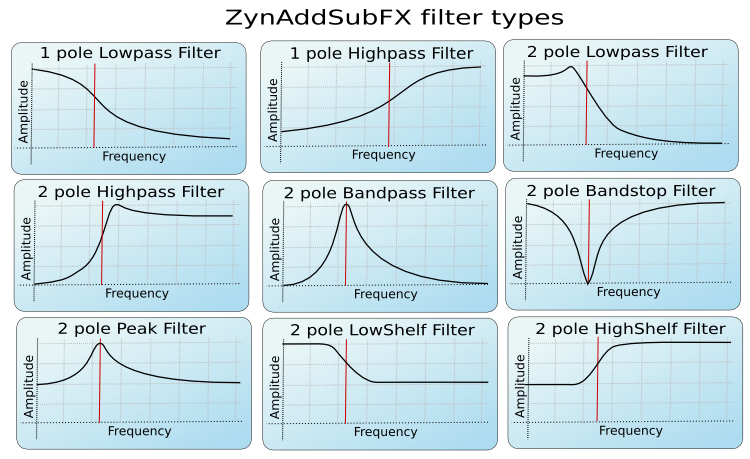
\includegraphics[scale=0.5]{zyn/zyn_filter_types_filter0.png}
   \caption[Basic Filter Types]{Filter Types, Yoshimi/ZynAddSubFX}
   \label{fig:basic_filter_types} 
\end{figure}

   \begin{enumber}
      \item A \textbf{low-pass} filter makes the sound more muffled.
      \item A \textbf{band-pass} filter makes the sound more tone-like, and
         sometimes more penetrating, if the total energy in the passband is
         preserved as the bandwidth decreases.
      \item A \textbf{high-pass} filter makes the sound seem sharper or more
         strident.
   \end{enumber}

\subsubsection{Filter Cutoff}
\label{subsubsec:filter_cutoff}

   \index{filter!cutoff}
   The filter cutoff value determines which frequency marks the changing
   point for the filter. In a low pass filter, this value marks the point
   where higher frequencies begin to be attenuated.

\subsubsection{Filter Resonance}
\label{subsubsec:filter_resonance}

   \index{filter!Q}
   \index{filter!resonance}
   The resonance of a filter determines how much excess energy is present at
   the cutoff frequency. In \textsl{Yoshimi} and \textsl{ZynAddSubFX},
   this is represented by the Q-factor,
   which is defined to be the cutoff frequency divided by the bandwidth. In
   other words higher Q values result in a much more narrow resonant spike.

   The Q value of a filter affects how concentrated
   the signal’s energy is at the cutoff frequency. The result of differing Q
   values are shown in \figureref{fig:low_q_vs_high_q}.
   For many classical analog sounds, high Q values were used on sweeping
   filters. A simple high Q low pass filter modulated by a strong envelope is
   usually sufficient to get a good sound.

\begin{figure}[H]
   \centering 
   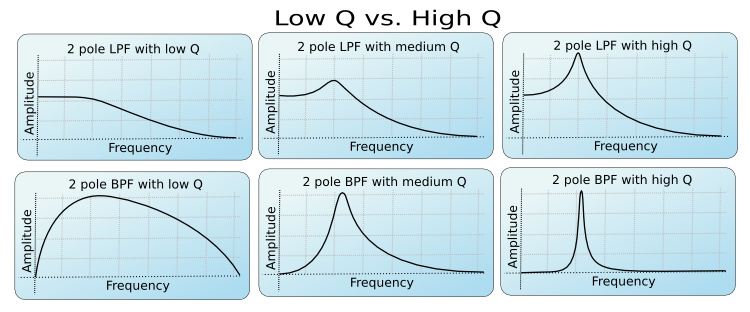
\includegraphics[scale=0.5]{zyn/low_q_high_q_filter1.png}
   \caption[Low Q vs. High Q]{The Effect of the Q Value}
   \label{fig:low_q_vs_high_q} 
\end{figure}

\subsubsection{Filter Stages}
\label{subsubsec:filter_stages}

   \index{filter!stages}
   \index{filter!order}
   The number of stages in a given filter describes how sharply it is able to
   make changes in the frequency response.
   The more stages, the sharper the filter.
   However, each added stage increases the processor time needed to make the
   filter calculation.

\begin{figure}[H]
   \centering 
   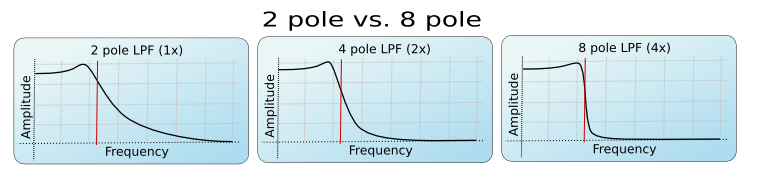
\includegraphics[scale=0.5]{zyn/2_pole_8_pole_filter2.png}
   \caption[2 Pole vs. 8 Pole Filter]{The Effect of the Order of a Filter}
   \label{fig:2_pole_vs_8_pole_filter}
\end{figure}

   The affect of the order of the filter can be seen in the figure above.
   This is roughly synonymous with the number of stages of the filter. For
   more complex patches, it is important to realize that the extra sharpness
   in the filter does not come for free, as it requires many more
   calculations to be performed. This phenomena is the most visible in
   SUBsynth, where it is easy to need several \textsl{hundred} filter stages
   to produce a given note.

   There are different types of filters. The number of poles define what will
   happen at a given frequency. Mathematically, the filters are functions which
   have poles that correspond to that frequency. Usually, two poles mean that
   the function has more "steepness", and that one can set the exact value of
   the function at the poles by defining the "resonance value". Filters with
   two poles are also often referred to as \textsl{Butterworth Filters}.

   For the interested, functions having poles means that we are given a
   quotient of polynomials. The denominator has degree 1 or 2, depending on the
   filter having one or two poles. In the file \texttt{DSP/AnalogFilter.cpp},
   \texttt{AnalogFilter :: computefiltercoefs()} sets the coefficients
   (depending on the filter type), and
   \texttt{AnalogFilter :: singlefilterout()} shows
   the whole polynomial (in a formula where no quotient is needed).

\subsubsection{Filter Parameters User Interface}
\label{subsubsec:filter_parameters_user_interface}

\begin{figure}[H]
   \centering 
   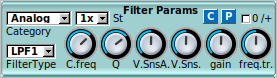
\includegraphics[scale=1.0]{subpanels/Filter_Params.png}
   \caption[Filter Parameters Sub-panel]{Stock Filter Parameters Sub-Panel}
   \label{fig:filter_parameters_subpanel} 
\end{figure}

   The user interface for filter parameters is a small stock sub-panel that
   is re-used in a number of larger dialog boxes, as shown in the figure
   above.  Let's describe each item of this sub-panel.

%  \figureref{fig:filter_parameters_subpanel}.

\begin{figure}[H]
   \centering 
   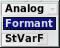
\includegraphics[scale=1.0]{bottom-panel/instrument-edit/ADD/filter-category.jpg}
   \caption[Filter Categories Dropdown]{Filter Categories, Dropdown Box}
   \label{fig:filter_categories_dropdown} 
\end{figure}

   \begin{enumber}
      \item \textbf{Category}
      \item \textbf{Filter Type}
      \item \textbf{C.freq}
      \item \textbf{Q}
      \item \textbf{V.SnsA}
      \item \textbf{freq.tr}
      \item \textbf{gain}
      \item \textbf{St}
      \item \textbf{C}
      \item \textbf{P}
   \end{enumber}

   \setcounter{ItemCounter}{0}      % Reset the ItemCounter for this list.

   \itempar{Category}{filter!category}
   Determines the category of filter to be used.
   There are three categories of filters
   (as shown in the dropdown element shown in
   \figureref{fig:filter_categories_dropdown}).

\begin{enumber}                     % enumber is our arabic numbering style
   \item \textbf{Analog} (the default)
   \item \textbf{Formant}
   \item \textbf{StVarF}
\end{enumber}

   An \textbf{analog} filter
   \index{filter!analog}
   is one that approximates a filter that is based on
   a network of resistors, capacitors, and inductors.

   A \textbf{formant} filter
   \index{filter!formant}
   is a more complex kind of filter that acts a lot
   like the human vocal tract, allowing for sounds that
   are a bit like human voices.

   A \textbf{state variable} ("StVarF") filter
   \index{filter!state variable}
   \index{filter!StVarF}
   \index{StVarF}
   is a type of active filter.
   The frequency of operation and the Q factor can be varied independently.
   This and the ability to switch between different filter responses make the
   state-variable filter widely used in analogue synthesizers.

   Values: \texttt{Analog*, Formant, StVarF}

   \itempar{Filter Type}{filter!type}
   Selects the type of filter to be used, such as high-pass, low-pass,
   and band-pass.
   See the dropdown element in \figureref{fig:filter_type_dropdown}.

\begin{figure}[H]
   \centering 
   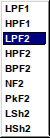
\includegraphics[scale=1.0]{bottom-panel/instrument-edit/ADD/filter-filtertype.jpg}
   \caption[Filter Type Dropdown]{Type of Filter Passband, Dropdown Box}
   \label{fig:filter_type_dropdown} 
\end{figure}

   Values: \texttt{LPF1, HPF1, LPF2*, HPF2, BPF2, NF2, PkF2, LSh2, HSh2}

   \itempar{C.freq}{cutoff frequency}
   \index{center frequency}
   Cutoff frequency or center frequency.
   This items has various definitions in the literature. 
   Usually it refers to the frequency at which the level
   drops to 3 Db below the maximum level.
   In various dialogs, this value is the
   center frequency of the filter or the base position in
   a vowel's sequence.

   Values: \texttt{0 to 127, 90*}

   \itempar{Q}{resonance level}
   The level of resonance for the filter. 
   It indicates a measure of the sharpness of a filter.
   The higher the Q, the sharper the filter.
   Generally, a higher Q value leads to a louder, more tonal
   affect for the filter.
   Note that some filter types might ignore this parameter.

   \itempar{V.SnsA}{velocity sensing amount}
   Velocity sensing amount for filter cutoff.
   Velocity sensing amount of the filter.

   Values: \texttt{0 to 127, 64*}

   \itempar{V.Sns}{velocity sensing function}
   \index{filter!velocity sensing function}
   Velocity sensing function of the filter.
   Set the amplitude of the velocity sensing.

   Values: \texttt{0 to 127, 64*}

   \itempar{freq.tr}{frequency tracking amount}
   \index{filter!frequency tracking amount}
   Filter Frequency Tracking Amount.
   When this parameter is positive, higher note
   frequencies shift the filter’s cutoff frequency higher.
   For the filter frequency tracking knob, left is negative, middle is
   zero, and right is positive.

   Values: \texttt{0 to 127, 64*}

   \itempar{gain}{filter!gain}
   Filter gain.
   Additional gain/attenuation for a filter.
   Also described as the filter output gain/damping factor.

   Values: \texttt{0 to 127, 64*}

   \itempar{St}{filter!stages}
   Filter stages.
   The more filter stages applied to a signal, the stronger (in general) the
   filtering.
   It is the number of additional times the filter will be applied (in
   order to create a very steep roll-off, such as 48 dB/octave).
   This dropdown
   element is shown in
   \figureref{fig:filter_stage_dropdown}.
   Obviously, the more stages used, the more calculation-intensive the
   filter will be.  This should also increase the latency (lag) of the
   filter.

\begin{figure}[H]
   \centering 
   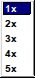
\includegraphics[scale=1.0]{bottom-panel/instrument-edit/ADD/filter-stages.jpg}
   \caption[Filter Stage Dropdown]{Filter Stage Dropdown}
   \label{fig:filter_stage_dropdown} 
\end{figure}

   Also present in this sub-panel are the usual \textbf{C}opy
   and \textbf{P}aste buttons that call up a copy-parameters or
   paste-parameters dialog.

\subsection{Stock Resonance Settings}
\label{subsec:stock_resonance_settings}

   \textsl{Yoshimi} provides for setting very arbitrary "resonance"
   settings for some sounds.  In fact, "resonance" is too limiting a word.
   A lot of control over the \textsl{spectrum} is possible.
   The following dialog is used by
   the ADDsynth editor,
   \figureref{subsec:addsynth_resonance}, and the
   the PADsynth editor,

   The resonance editor is brought on-screen via the
   \textbf{Resonance} button of the ADDsynth or PADsynth
   global part editors.

   The resonance effect acts as a "resonance box" or a filter with arbitrary
   frequency response. This produces very realistic sounds. 
   The cursor location is shown below the graph (the frequency, kHz, and
   the amplitude, dB). 

   Paul Nasca has a video on YouTube that includes a demonstration of how
   the resonance dialog works and affects the sound, if you care to look for
   it.

\begin{figure}[H]
   \centering 
   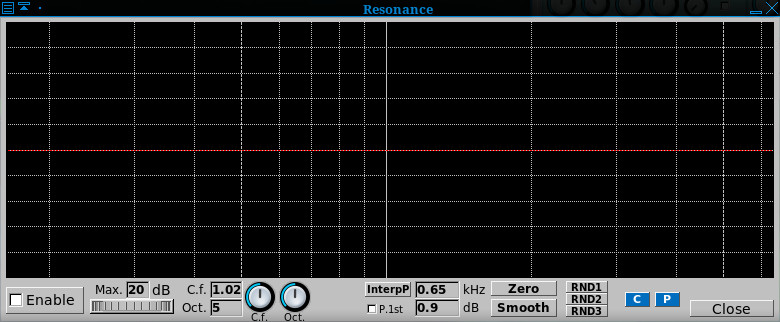
\includegraphics[scale=0.75]{bottom-panel/instrument-edit/ADD/ADDsynth-resonance.jpg}
   \caption{ADDsynth/PADsynth Resonance}
   \label{fig:addsynth_resonance}
\end{figure}

   \begin{enumber}
      \item \textbf{Graph Window}
      \item \textbf{Enable}
      \item \textbf{Max dB (wheel)}
      \item \textbf{C.f. (knob)}
      \item \textbf{Oct.}
      \item \textbf{P.1st}
      \item \textbf{InterpP}
      \item \textbf{KHz}
      \item \textbf{dB}
      \item \textbf{Zero}
      \item \textbf{Smooth}
      \item \textbf{RND1}
      \item \textbf{RND2}
      \item \textbf{RND3}
      \item \textbf{C}
      \item \textbf{P}
      \item \textbf{Close}
   \end{enumber}

   \setcounter{ItemCounter}{0}      % Reset the ItemCounter for this list.

   \itempar{Graph Window}{resonance!graph}
   Resonance Graph Window.
   Lets one draw the resonance frequency response in "freehand" mode.

   \itempar{Enable}{resonance!Enable}
   Resonance Enable.
   Turn the Resonance effect on.

   Values: \texttt{Off*, On}

   \itempar{Max dB (wheel)}{resonance!max db}
   The Maximum Amplitude (dB) wheel.
   Sets the amount of resonance: lower values have little effect. Use the
   roller below to set it. 

   Values: \texttt{1 to 90, 20*}

   \itempar{C.f. (knob)}{resonance!cf}
   Center Frequency (kHz).
   Sets the center frequency of the graph.
   The value is shown in the read-only text-box to the left.

   Values: \texttt{0 to 127, 64*} for \texttt{0.10 to 10.0, 1.0*}

   \itempar{Oct}{resonance!octaves}
   Number of Octaves.
   Sets the number of octaves the graph represents.
   The value is shown in the read-only text-box to the left.

   Values: \texttt{0 to 127, 64*} for \texttt{0 to 10, 5*}

   \itempar{P.1st}{resonance!first harmonic}
   Protect the fundamental Frequency.
   Do not damp the first harmonic.
   What does this mean, what affect does it have?
   \index{todo!first harmonic}

   Values: \texttt{Off, On}

   \itempar{InterpP}{resonance!interpolate}
   Interpolate the peaks.
   This setting is a weird one where mouse movement affects it,
   but also affects the next field as well.  Oh, kHz and dB.

   This setting allows one to make resonance functions very easily.  To use
   it effectively, first, clear the graph using the \textbf{Zero} button.
   Click the left button on a position on the graph. Click the
   \textbf{InterpP} button. It will interpolate automatically between the
   positions pointed to (or drew).  Also one can clear a part of the graph
   by dragging with the right mouse button. In fact, the \textbf{interpP}
   button interpolates between non-zero values.  If one presses the
   \textbf{InterpP} with the right mouse button, the interpolation will be
   linear, and if one uses the left button, the interpolation will be
   smooth. 

   \itempar{KHz}{resonance!khz}
   The current frequency on graph.

   \itempar{dB}{resonance!db}
   The current level on graph window.

   Values: \texttt{-90 to +90}

   \itempar{Zero}{resonance!clear}
   Clear the resonance function.
   Zero. Clear the graph.

   Amplification - how the output signal is amplified (WHERE?)

   \itempar{Smooth}{resonance!smooth}
   Smooth the resonance function.
   Smooth the graph.

   TODO:  What is the exact nature of this smoothing?
   \index{todo!resonance smooth}

   \itempar{RND1}{resonance!randomize}
   Randomize the resonance function, 1.
   RND1, RND2, RND3 are used to create random resonance functions.

   \itempar{RND2}{resonance!randomize}
   Randomize the resonance function, 2.

   \itempar{RND3}{resonance!randomize}
   Randomize the resonance function, 3.

   \itempar{C}{resonance!copy}
   Copy Dialog.

   \itempar{P}{resonance!paste}
   Paste Dialog.

   \itempar{Close}{resonance!close}
   Close.

\subsection{LFO Settings}
\label{subsec:lfo_settings}

   \textsl{Yoshimi} provides LFOs for it amplitude, frequency, and filtering
   functions.
   "LFO" means Low Frequency Oscillator. These oscillators are not used to make
   sounds by themselves, but they change parameters cyclically as a sound
   plays.

   LFOs are, as the name says, oscillators with, compared to the frequency of
   the sound, low frequency. They often appear in order to control the
   effect.

\subsubsection{LFO Basic Parameters}
\label{subsubsec:lfo_basic_parameters}

\begin{figure}[H]
   \centering 
   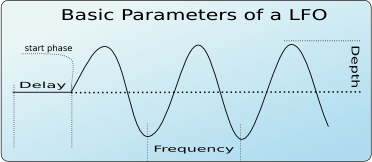
\includegraphics[scale=0.75]{zyn/basic_parameters_lfo0.png}
   \caption[Basic LFO Parameters]{Basic LFO Parameters}
   \label{fig:basic_parameters_lfo} 
\end{figure}

   \begin{enumber}
      \item \textbf{Delay}.
      \item \textbf{Start Phase}.
      \item \textbf{Frequency}.
      \item \textbf{Depth}.
   \end{enumber}

   The LFOs has some basic parameters (see
   \figureref{fig:basic_parameters_lfo}.

   \setcounter{ItemCounter}{0}      % Reset the ItemCounter for this list.

   \itempar{Delay}{LFO!delay}
   LFO Delay.
   This parameter sets how much time takes since the start of the note to
   start the cycling of the LFO.
   When the LFO starts, it has a certain position called "start phase".

   \itempar{Start Phase}{LFO!start phase}
   LFO Start Phase.
   The angular position at which a LFO waveform will start.

   \itempar{Frequency}{LFO!frequency}
   LFO Frequency.
   How fast the LFO is (i.e. how fast the parameter controlled by
   the LFO changes.)

   \itempar{Depth}{LFO!depth}
   LFO Depth.
   The amplitude of the LFO (i.e. how much the parameter is controlled by
   the LFO changes.)

\subsubsection{LFO Function}
\label{subsubsec:lfo_function}

   \index{LFO!shape}
   \index{LFO!type}
   \index{LFO!function}
   Another important additional LFO parameter is the shape or type of the
   LFO. There are many LFO Types that vary according to the function used to
   generate the LFO. \textsl{Yoshimi} supports the LFO shapes shown in
   \figureref{fig:types_of_lfo}.

\begin{figure}[H]
   \centering 
   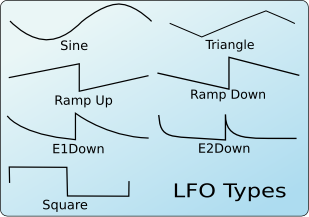
\includegraphics[scale=0.75]{zyn/types_of_lfo1.png}
   \caption[LFO Functions]{LFO Types, Shapes, or Functions}
   \label{fig:types_of_lfo}
\end{figure}

\subsubsection{LFO Randomness}
\label{subsubsec:lfo_randomness}

\begin{figure}[H]
   \centering 
   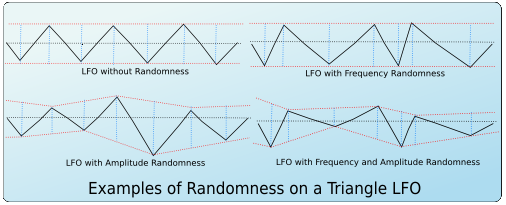
\includegraphics[scale=0.75]{zyn/randomness_in_lfo2.png}
   \caption[LFO Randomization]{LFO Randomization}
   \label{fig:randomness_in_lfo}
\end{figure}

   \index{LFO!randomness}
   Another parameter is the LFO Randomness. It modifies the LFO amplitude or
   the LFO frequency at random. In \textsl{Yoshimi}
   one can choose how much the LFO
   frequency or LFO amplitude changes by this parameter.
   Observe \figureref{fig:randomness_in_lfo}.
   It shows some examples of randomness and how it changes the shape of a
   triangle LFO.

\subsubsection{LFO, More Settings}
\label{subsubsec:lfo_more_settings}

   Other settings are available as well.

   \index{LFO!continuous mode}
   Continous mode: If this mode is used, the LFO will not start from "zero" on
   each new note, but it will be continuous. This is very useful if one
   applies on filters to make interesting sweeps.

   \index{LFO!stretch}
   Stretch: It controls how much the LFO frequency changes according to the
   note’s frequency. It can vary from negative stretch (the LFO frequency is
   decreased on higher notes) to zero (the LFO frequency will be the same
   on all notes) to positive stretch (the LFO frequency will be
   increased on higher notes).

\subsubsection{LFO User Interface Panels}
\label{subsubsec:lfo_user_interface_panels}

   \setcounter{ItemCounter}{0}      % Reset the ItemCounter for this list.

\begin{figure}[H]
   \centering 
   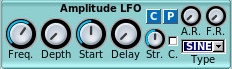
\includegraphics[scale=1.0]{subpanels/Amplitude_LFO.png}
   \caption[Amplitude LFO Sub-Panel]{Amplitude LFO Sub-Panel}
   \label{fig:amplitude_lfo}
\end{figure}

   In \textsl{Yoshimi}, LFO parameters are available for amplitude, filters,
   and frequency.  They all have essentially the same interface elements.
   Note \figureref{fig:amplitude_lfo}, which
   shows an example of an LFO stock sub-panel.

These parameters are:

   \begin{enumber}
      \item \textbf{Freq}
      \item \textbf{Depth}
      \item \textbf{Start}
      \item \textbf{Delay}
      \item \textbf{A.R}
      \item \textbf{F.R}
      \item \textbf{C} or \textbf{C.}
      \item \textbf{Str}
      \item \textbf{Type}
      \item \textbf{C} (copy)
      \item \textbf{P} (paste)
   \end{enumber}

   \setcounter{ItemCounter}{0}      % Reset the ItemCounter for this list.

   \itempar{Freq}{LFO!frequency}
   LFO Frequency.
   This parameter varies from 0 to 1.
   We still need to figure out what that scale means, however.
   Obviously, it is a relative scale, and is perhaps related to the
   overall sampling frequency.

   Values: \texttt{0 to 1, 0.63*}

   \itempar{Depth}{LFO!depth}
   \index{LFO!amount}
   LFO Depth.  Also called "LFO Amount".

   Values: \texttt{0* to 127}

   \itempar{Start}{LFO!starting phase}
   LFO Start Phase. If this knob is at the lowest value, the LFO Start
   Phase will be random.

   Values: \texttt{0 = random, to 127, 64*}

   \itempar{Delay}{LFO!delay}
   LFO Delay.

   Values: \texttt{0* to 127}

   \itempar{A.R}{LFO!amplitude randomness}
   LFO Amplitude Randomness.

   Values: \texttt{0* to 127}

   \itempar{F.R}{LFO!frequency randomness}
   LFO Frequency Randomness.

   Values: \texttt{0* to 127}

   \itempar{C}{LFO!continuous mode}
   LFO Continous Mode.

   Values: \texttt{Off*, On}

   \itempar{Str}{LFO!stretch}
   LFO Stretch. See the image in
   \figureref{fig:amplitude_lfo}.
   It shows that the LFO stretch is set to zero,
   though the tooltip would show it to be 64.

   Values: \texttt{0 to 127, 64*}

   \itempar{Type}{LFO!type}
   LFO Function.
   Also present in this sub-panel are the usual \textbf{C}opy
   and \textbf{P}aste buttons that call up a copy-parameters or
   paste-parameters dialog.

   Values: \texttt{SINE*, TRI, SQR, R.up, R.dn, E1dn, E2dn}

\begin{figure}[H]
   \centering 
   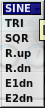
\includegraphics[scale=1.0]{bottom-panel/instrument-edit/ADD/lfo-function-type.jpg}
   \caption[LFO Type Drop-down]{LFO Function Type Drop-down}
   \label{fig:lfo_function_type_dropdown}
\end{figure}

   \itempar{Type}{LFO!function type}
   LFO Type (or Shape, or Function).
   The various shapes of LFO functions are shown in
   \figureref{fig:types_of_lfo}.
   The values that can be selected are shown in
   \figureref{fig:lfo_function_type_dropdown}.
   Also present in this sub-panel are the usual \textbf{C}opy
   and \textbf{P}aste buttons that call up a copy-parameters or
   paste-parameters dialog.

   Values: \texttt{SINE*, TRI, SQR, R.up, R.dn, E1dn, E2dn}

   For reference,
   \figureref{fig:filter_lfo}
   shows the LFO sub-panel for a filter, and
   \figureref{fig:frequency_lfo_subpanel}
   shows the LFO sub-panel for frequency.

\subsubsection{Filter LFO Sub-panel}
\label{subsubsec:filter_lfo_sub_panel}

   % Obtain sub-items from checklist

\begin{figure}[H]
   \centering 
   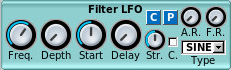
\includegraphics[scale=1.0]{subpanels/Filter_LFO.png}
   \caption[Filter LFO Sub-Panel]{Filter LFO Sub-Panel}
   \label{fig:filter_lfo}
\end{figure}

   \begin{enumber}
      \item \textbf{Enable} (present on some versions of this sub-panel).
      \item \textbf{Freq.}
      \item \textbf{Depth}
      \item \textbf{Start}
      \item \textbf{Delay}
      \item \textbf{Str.}
      \item \textbf{C.}
      \item \textbf{A.R.}
      \item \textbf{F.R.}
      \item \textbf{Type}
      \item \textbf{C}
      \item \textbf{P}
   \end{enumber}

   \setcounter{ItemCounter}{0}      % Reset the ItemCounter for this list.

   \itempar{Enable}{lfo!enable}
   Enable the panel.  (Present on some versions of this sub-panel).

   \itempar{Freq}{lfo!frequency}
   LFO Frequency.

   Values: \texttt{0 to 1, 0.64*}

   \itempar{Depth}{lfo!depth}
   LFO Amount.

   Values: \texttt{0* to 127}

   \itempar{Start}{lfo!start phase}
   LFO Startphase (leftmost is random).

   Values: \texttt{0 to 127, 64*}

   \itempar{Delay}{lfo!delay}
   LFO Delay.

   Values: \texttt{0* to 127}

   \itempar{Str}{lfo!stretch}
   LFO Stretch.

   Values: \texttt{0 to 127, 64*}

   \itempar{C}{lfo!continuous}
   Continuous LFO.

   Values: \texttt{Off*, On}

   \itempar{A.R}{lfo!random amplitude}
   LFO Amplitude Randomness.

   Values: \texttt{0* to 127}

   \itempar{F.R}{lfo!random frequency}
   LFO Frequency Randomness.

   Values: \texttt{0* to 127}

   \itempar{Type}{lfo!type}
   LFO Type.

\begin{figure}[H]
   \centering 
   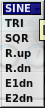
\includegraphics[scale=1.0]{bottom-panel/instrument-edit/ADD/lfo-function-type.jpg}
   \caption[LFO Function Types]{LFO Function Type Dropdown}
   \label{fig:frequency_lfo_dropdown}
\end{figure}

   Values: \texttt{SINE*, TRI, SQR, R.up, R.dn, E1dn, E2dn}

   \itempar{C}{lfo!copy}
   Copy to Clipboard/Preset.

   \itempar{P}{lfo!paste}
   Paste from Clipboard/Preset.

\subsubsection{Frequency LFO Sub-panel}
\label{subsubsec:frequency_lfo_sub_panel}

\begin{figure}[H]
   \centering 
   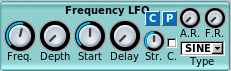
\includegraphics[scale=1.0]{subpanels/Frequency_LFO.png}
   \caption[Frequency LFO Sub-Panel]{Frequency LFO Sub-Panel}
   \label{fig:frequency_lfo_subpanel}
\end{figure}

   This panel is basically identical to the Filter LFO panel described
   in the previous section.

% Move this section upward?

\subsection{Envelope Settings}
\label{subsec:envelope_settings}

   Envelopes control how the amplitude, the frequency, or the filter changes
   over time.  The general envelope generator has four sections:

   \begin{enumber}
      \item \textbf{Attack}.
         \label{ref:attack}
         \index{attack}
         \index{envelope!attack}
         The attack is the initial envelope response. 
         It begins when the key for the note is first held down
         (at Note On).
         The volume starts at 0, and rises fast or slowly until a peak value.
         In \textsl{Yoshimi}, the attack is always linear.
      \item \textbf{Decay}
         \label{ref:decay}
         \index{decay}
         \index{envelope!decay}
         When the attack is at its highest value, it immediately begins
         to decay to the sustain value.  The decay can be fast or slow.
         The attack and decay together can be used to produce something like
         horn blips, for example.
      \item \textbf{Sustain}
         \label{ref:sustain}
         \index{sustain}
         \index{envelope!sustain}
         This is the level at which the parameter stays while the key is
         held down, i.e. until a Note Off occurs.
      \item \textbf{Release}
         \label{ref:release}
         \index{release}
         \index{envelope!release}
         When the key is released, the sound decays, either fast or slowly,
         until it is off (the volume is 0).
   \end{enumber}

   Together, these values are called "ADSR".  
   The ADSR envelope generally controls the amplitude of the sound.
   In \textsl{Yoshimi},
   amplitude envelopes can be \textsl{linear} or \textsl{logarithmic}.

\begin{figure}[H]
   \centering 
   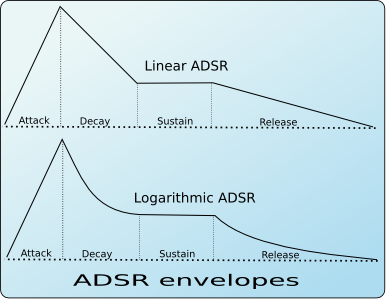
\includegraphics[scale=0.75]{zyn/ADSR_envelope1.png}
   \caption{ADSR Envelope (Amplitude)}
   \label{fig:adsr_envelope_depiction}
\end{figure}

   See \figureref{fig:adsr_envelope_depiction},
   it shows a depiction of an ADSR envelope.
   The ADSR is mostly applied to amplitude envelopes.

\begin{figure}[H]
   \centering 
   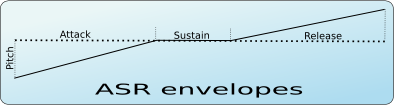
\includegraphics[scale=0.75]{zyn/ASR_frequency_envelope2.png}
   \caption{ASR Envelope, Frequency}
   \label{fig:asr_envelope_depiction}
\end{figure}

   Frequency envelopes control the frequency (more exactly, the pitch) of the
   oscillators. The following image depicts the stages of these envelopes.

   For frequency envelopes, a simpler form of envelope is used.
   This envelope is an ASR envelope, shown in
   \figureref{fig:asr_envelope_depiction}.
   The dotted line represents the real pitch of the sound without the envelope.
   The frequency envelopes are divided into 3 stages:

   \begin{enumber}
      \item \textbf{Attack}. 
      It begins at the Note On. The frequency starts from a certain value and
      glides to the real frequency of the note.
      \item \textbf{Sustain}.
      The frequency stays the same during the sustain period.
      \item \textbf{Release}.
      This stage begins on Note Off and glides the frequency of the note to a
      certain value.
   \end{enumber}

\subsubsection{Amplitude Envelope Sub-Panel}
\label{subsubsec:amplitude_envelope_subpanel}

\begin{figure}[H]
   \centering 
   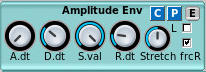
\includegraphics[scale=1.0]{subpanels/Amplitude_Env.png}
   \caption[Amplitude Envelope Sub-Panel]{Amplitude Envelope Sub-Panel}
   \label{fig:amplitude_env}
\end{figure}

   \begin{enumber}
      \item \textbf{A.dt}
      \item \textbf{D.dt}
      \item \textbf{S.val}
      \item \textbf{R.dt}
      \item \textbf{Str}
      \item \textbf{L}
      \item \textbf{frcR}
      \item \textbf{C}
      \item \textbf{P}
      \item \textbf{E}
   \end{enumber}

   \setcounter{ItemCounter}{0}      % Reset the ItemCounter for this list.

   \itempar{A.dt}{envelope!attack time}
   Attack duration, attack time.
   We need to determine the units of time at play for ADSR durations.

   Values: \texttt{0* to 127}

   \itempar{D.dt}{envelope!decay time}
   Decay duration, decay time.

   Values: \texttt{0 to 127, 44*}

   \itempar{S.val}{envelope!sustain value}
   Sustain value.
   This is the (relative?) level at which the envelope will settle
   while the note is held down.
   The only stage that always remains defined is the Sustain, where the
   envelopes freezes until a Note Off event.

   Values: \texttt{0 to 127*}

   \itempar{R.dt}{envelope!release time}
   Release time.

   Values: \texttt{0 to 127, 25*}

   \itempar{Str}{envelope!stretch}
   Stretch.
   How the envelope is stretched according the note.
   Envelope Stretch means that, on lower notes, the envelope will be longer.
   On the higher notes the envelopes are shorter than lower notes. In the
   leftmost value, the stretch is zero. The rightmost use a stretch of 200\%;
   this means that the envelope is stretched about 4 times per octave.

   Values: \texttt{0 to 127, 64*}

   \itempar{L}{envelope!linear}
   Linear envelope.
   If this option is set, the envelope is linear, otherwise, it will be
   logarithmic.

   Values: \texttt{Off*, On}

   \itempar{frcR}{envelope!forced release}
   Forced release.
   This means that if this option is turned on, the release will go to the
   final value, even if the sustain stage is not reached. Usually, this must
   be set.
   If this option is turned on, the release will go to the
   final value, even if the sustain level is not reached.
   Also present in this sub-panel are the usual \textbf{C}opy
   and \textbf{P}aste buttons that call up a copy-parameters or
   paste-parameters dialog.

   Values: \texttt{Off, On*}

   \itempar{C}
   Copy to Clipboard/Preset.

   \itempar{P}
   Paste from Clipboard/Preset.

   \itempar{E}
   Amplitude Envelope Editing Window.
   Described in the next section.

\subsubsection{Envelope Settings}
\label{subsubsec:envelope_settings}

   This section describes the \textbf{Amplitude Envelope Editing} window.

\begin{figure}[H]
   \centering 
   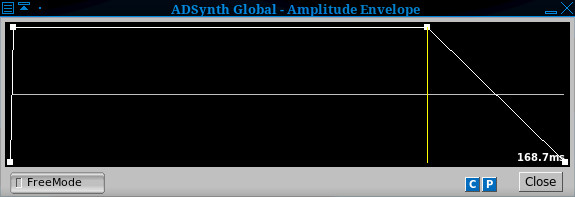
\includegraphics[scale=1.0]{bottom-panel/instrument-edit/ADD/amplitude-envelope.jpg}
   \caption{Amplitude/Filter/Frequency Envelope Editor}
   \label{fig:amplitude_envelope_editor}
\end{figure}

   \begin{enumber}
      \item \textbf{Graph Window}
      \item \textbf{FreeMode}
      \item \textbf{C}
      \item \textbf{P}
      \item \textbf{Close}
   \end{enumber}

   \setcounter{ItemCounter}{0}      % Reset the ItemCounter for this list.

   \itempar{FreeMode}{envelope!freemode enable}
   Freemode Enable.
   Enables the envelope editor's Free Mode.
   See the next section for details.

   Values: \texttt{Off*, On} \\

\subsubsection{Freemode Envelope Settings}
\label{subsubsec:freemode_envelope_settings}

   The envelope panels are parts that control a parameter (such as the
   frequencies) of a sound.  For all envelopes, there is a mode that allows the
   user to set an arbitrary number of stages and control points. This mode is
   called \textsl{Freemode}.  The only stage that always remains defined is the
   Sustain, where the envelopes freezes until a Note Off event.  The Freemode
   envelope editor has a separate window to set the parameters and controls.

   The main concept of the freemode editor window is the
   \textsl{control point}.
   \index{control point}
   One can move the points using the mouse. In the right on the
   window, it shows the total duration of the envelope. If the mouse button
   is pressed on a control point, it will be shown the duration of the
   stage where the point is.

   \figureref{fig:amplitude_envelope_freemode}
   shows an example of the stock Freemode envelope editor, with
   Freemode enabled.

\begin{figure}[H]
   \centering 
   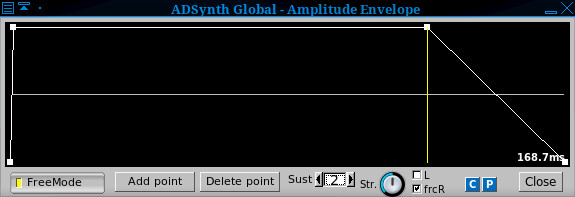
\includegraphics[scale=1.0]{bottom-panel/instrument-edit/ADD/amplitude-envelope-freemode.jpg}
   \caption{Amplitude/Filter/Frequency Envelope Freemode Editor}
   \label{fig:amplitude_envelope_freemode}
\end{figure}

   All of the envelope editors have some common controls.

   \begin{enumber}
      \item \textbf{Graph Window}
      \item \textbf{Add point}
      \item \textbf{E}
      \item \textbf{FreeMode}
      \item \textbf{Add point}
      \item \textbf{Delete point}
      \item \textbf{Sust}
      \item \textbf{Stretch}
      \item \textbf{L}
      \item \textbf{frcR}
      \item \textbf{Close}
      \item \textbf{C}
      \item \textbf{P}
   \end{enumber}

   \setcounter{ItemCounter}{0}      % Reset the ItemCounter for this list.

   \itempar{E}{envelope!editor}
   Editor.  Graph Window.
   Shows a window with the real envelope shape and the option to convert to
   Freemode to edit it.
   The envelope editor shows a window in which one can view and modify the
   detailed envelope shape, or convert it to Freemode to edit it almost
   without restriction.
   By default, only the \textsl{Freemode} button/checkbox is visible.

   If an envelope has FreeMode enabled, it allows one to edit the
   graph of the envelope directly. Select a point from the graph and move it.
   Notice that
   \textsl{only the line \textbf{before} the currently edited point of the
   envelope} changes its duration.
   As the point is dragged, the text on the right shows the duration of
   the line before it. Otherwise, the text shows the total duration of the
   envelope. 

   If the envelope doesn't have the FreeMode mode enabled, it doesn't allow
   one to move the points; the envelope window is then useful only to see
   what happens if one changes the ADSR settings.

   \itempar{FreeMode}{envelope!freemode}
   FreeMode.  Provides a mode where completely arbitrary envelopes may be
   drawn.
   Actually, the envelopes aren't completely arbitrary, as the sustain
   section is always flat, and its duration corresponds with the duration
   the note is held down.
   When this mode is enabled, the rest of the controls shown in
   \figureref{fig:amplitude_envelope_freemode}
   appear, and are described in the following paragraphs.

   Values: \texttt{Off*, On}

   \itempar{Add point}{envelope!add point}
   Add point.
   Provides a way to add a data point to the Freemode envelope.
   It adds the point after the currently-selected point. One can select a
   point by clicking on it.

   \itempar{Delete point}{envelope!delete point}
   Delete point.
   Provides a way to delete the current data point from the Freemode envelope.

   \itempar{Sust}{envelope!sustain}
   Sustain point.
   Sets the sustain point.
   The sustain point is shown using the yellow line.
   If the point is at 0, then sustain is disabled.
   It is difficult to determine the difference between 1 and 2.

   \begin{enumber}
      \item{0} means that sustain is disabled, and the envelope immediately
      starts dying, even if the note is held.
      \item{1} seems to mean the sustain curve follows its course while the
      note is held.
      \item{2} seems to mean that extra sustain kicks in after the note is
      released.
   \end{enumber}

   Values: \texttt{0, 1, 2*}

   \itempar{Stretch}{envelope!stretch}
   Envelope Stretch.
   How the envelope is stretched according the note. On the higher notes the
   envelopes are shorter than lower notes. At the leftmost value, the
   stretch is zero. The rightmost sets a stretch of 200\%; this means that the
   envelope is stretched about four times/octave.

   \itempar{L}{envelope!linear}
   Envelope Linear.
   This setting is only available in the amplitude envelope.
   If enabled, the envelope is linear.
   If not enabled, the envelope is logarithmic (dB).

   Values: \texttt{Off*, On}

   \itempar{frcR}{envelope!forced release}
   Forced Release.
   This means that if this option is turned on, the release will go
   immediately to the final value, even if the sustain stage is not reached.
   Usually, this must be set.
   When the key is released, the position of the envelope jumps directly to
   the point after the release point. If the release is disabled, the
   envelope position jumps to the last point on release.

   Values: \texttt{Off*, On}

   \itempar{Close}{envelope!close dialog}
   Close Dialog.

   Also present in this sub-panel are the usual \textbf{C}opy
   and \textbf{P}aste buttons that call up a copy-parameters or
   paste-parameters dialog, as well as a button
   to bring up the editor window.

\subsubsection{Envelope Settings, Frequency}
\label{subsubsec:envelope_settings_for_frequency}

   These envelopes controls the frequency (more exactly, the pitch) of the
   oscillators.
   Observe \figureref{fig:asr_envelope_depiction}.
   It depicts the stages of these envelopes.
   The dotted line represents the real pitch of the sound without the envelope.

   The frequency envelopes are divided into 3 stages:
   attack (see \ref{ref:attack});
   sustain (see \ref{ref:sustain});
   and
   release (see \ref{ref:release}).

   One question to answer is:  
   can the attack and release go in the opposite directions, or do the knob
   ranges prohibit this?

\begin{figure}[H]
   \centering 
   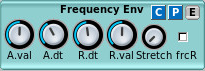
\includegraphics[scale=1.0]{subpanels/Frequency_Env.png}
   \caption[Frequency Envelope Sub-Panel]{Frequency Envelope Sub-Panel}
   \label{fig:frequency_env}
\end{figure}

   \begin{enumber}
      \item \textbf{Enable} (present on some versions of this sub-panel).
      \item \textbf{A.value} or \textbf{A.val}
      \item \textbf{A.dt}
      \item \textbf{R.dt}
      \item \textbf{R.val} (present on some versions of this sub-panel).
      \item \textbf{Stretch}
      \item \textbf{frcR}
      \item \textbf{C}
      \item \textbf{P}
      \item \textbf{E}
   \end{enumber}

   For Frequency Envelopes the interface has the following parameters:

   \setcounter{ItemCounter}{0}      % Reset the ItemCounter for this list.

   \itempar{Enable}{envelope!enable}
   Enable the panel.  (Present on some versions of this sub-panel).

   \itempar{A.val}{envelope!attack value}
   Attack value.
   We need to figure out what this means.

   Values: \texttt{0 to 127, 64*}

   \itempar{A.dt}{envelope!attack time}
   Attack duration. Attack time.

   Values: \texttt{0 to 127, 40*}

   \itempar{R.dt}{envelope!release time}
   Release time.

   Values: \texttt{0 to 127, 60*}

   \itempar{R.val}{envelope!release value}
   Release Value.
   Actually present only on the Frequency Env sub-panel.

   Values: \texttt{0 to 127, 64*}

   \itempar{Stretch}{envelope!stretch}
   Envelope Stretch.
   Envelope Stretch (on lower notes make the envelope longer).

   Values: \texttt{0 to 127, 64*}

   \itempar{frcR}{envelope!forced release}
   Forced release.
   If this option is turned on, the release will go to the
   final value, even if the sustain level is not reached.

   Values: \texttt{Off, On*}

   Also present in this sub-panel are the usual \textbf{C}opy
   and \textbf{P}aste buttons that call up a copy-parameters or
   paste-parameters dialog, as well as a button
   to bring up the editor window.

\subsubsection{Envelope Settings for Filter}
\label{subsubsec:envelope_settings_for_filter}

   This envelope controls the cutoff frequency of the filters.
   The filter envelopes are divided into 4 stages:

   \begin{enumber}
      \item \textbf{Attack}.
         It begins at the Note On.
         The cutoff frequency starts from a certain value and glides to another
         value.
      \item \textbf{Decay}.
         The cutoff frequency continues to glide to the real cutoff frequency
         value of the filter (dotted line).
      \item \textbf{Sustain}.
         The cutoff frequency stays the same during the sustain period (dotted
         line).
      \item \textbf{Release}.
         This stage begins on Note Off and glides the filter cutoff frequency
         of the note to a certain value.
   \end{enumber}

\begin{figure}[H]
   \centering 
   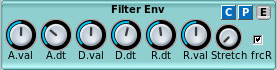
\includegraphics[scale=1.0]{subpanels/Filter_Env.png}
   \caption[Filter Envelope Sub-Panel]{Filter Envelope Sub-Panel}
   \label{fig:filter_env}
\end{figure}

   \begin{enumber}
      \item \textbf{A.value}
      \item \textbf{A.dt}
      \item \textbf{D.val}
      \item \textbf{D.dt}
      \item \textbf{R.dt}
      \item \textbf{Stretch}
      \item \textbf{frcR}
      \item \textbf{L}
   \end{enumber}

   Filter Envelopes has the following parameters:

   \setcounter{ItemCounter}{0}      % Reset the ItemCounter for this list.

   \itempar{A.value}{envelope!attack value}
   Attack Value.  Starting Value.
   We need to figure out what this means.

   Values: \texttt{0 to 127, 64*}

   \itempar{A.dt}{envelope!attack time}
   Attack Duration.  Attack Time.

   Values: \texttt{0 to 127, 40*}

   \itempar{D.val}{envelope!decay value}
   Decay Value.

   Values: \texttt{0 to 127, 64*}

   \itempar{D.dt}{envelope!decay time}
   Decay Duration.  Decay Time.

   Values: \texttt{0 to 127, 70*}

   \itempar{R.dt}{envelope!release time}
   Release time.

   Values: \texttt{0 to 127, 60*}

   \itempar{Stretch}{envelope!stretch}
   Stretch.
   Envelope Stretch (on lower notes make the envelope longer).

   Values: \texttt{0 to 127, 64*}

   \itempar{frcR}{envelope!forced release}
   Forced Release.
   If this option is turned on, the release will go to the
   final value, even if the sustain level is not reached.

   Values: \texttt{Off, On*}

   Also present in this sub-panel are the usual \textbf{C}opy
   and \textbf{P}aste buttons that call up a copy-parameters or
   paste-parameters dialog, as well as a button that bring up the editor
   window.

%  Additional picture and GUI items for ADDsynth version?
%  Figure: bottom-panel/instrument-edit/ADD/ADDsynth-filter-envelope.jpg

   \itempar{L}{envelope!linearity}
   If this option is set, the envelope is linear, otherwise, it will be
   logarithmic.

   Values: \texttt{Off*, On}

\subsubsection{Formant Filter Settings}
\label{subsubsec:formant_filter_settings}

   This window allows one to change most of the parameters of the formant
   filter.   It is reached by enabling a \textbf{FILTER} panel,
   changing the \textbf{Category} value to \textsl{Formant}, and then clicking
   the \textbf{Edit} button that sits below the category drop-down list.

\begin{figure}[H]
   \centering 
%  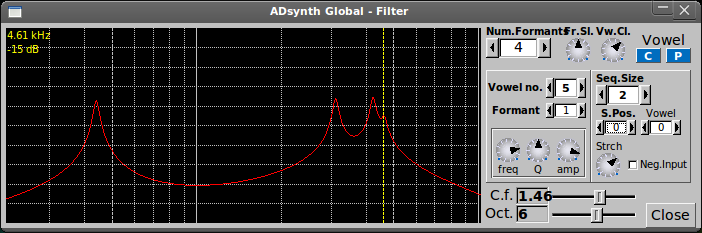
\includegraphics[scale=0.75]{zyn/formant_filter.png}
   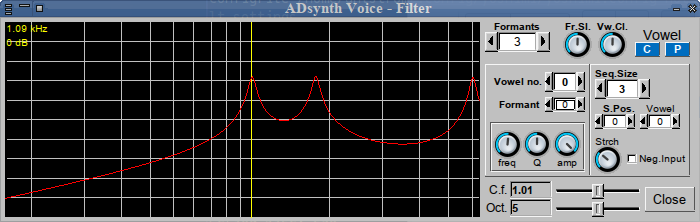
\includegraphics[scale=1.0]{subpanels/addsynth_voice_formant_filter.png}
   \caption[Formant Filter Editor]{Formant Filter Editor Dialog}
   \label{fig:formant_filter_editor}
\end{figure}

   This editor dialog provides a lot of functionality:

   \begin{enumber}
      \item \textbf{Formants}
      \item \textbf{Fr.Sl.}
      \item \textbf{Vw.Cl.}
      \item \textbf{C.f.}
      \item \textbf{Oct.}
      \item \textbf{Vowel no.}
      \item \textbf{Formant}
      \item \textbf{freq}
      \item \textbf{Q}
      \item \textbf{amp}
      \item \textbf{Seq.Size}
      \item \textbf{S.Pos.}
      \item \textbf{Vowel}
      \item \textbf{Strtch}
      \item \textbf{Neg Input}
   \end{enumber}

\paragraph{Formant Parameters}
\label{paragraph:formant_parameters}

   \itempar{Formants}{formants!number of}
   Number of Formants Used.

   Values:  \texttt{1 to 12, 3*}

   \itempar{Fr.Sl}{formants!slowness}
   Formant Slowness.
   This parameters prevents too-fast morphing between vowels.

   Values:  \texttt{0 to 127, 64*}

   \itempar{Vw.Cl}{formants!vowel clearness}
   Vowel "Clearness".
   Sets how much the vowels are kept "clear",
   that is, how much "mixed" vowels are avoided.

   Values:  \texttt{0 to 127, 64*}

   \itempar{C.f}{formants!cf}
   Center Frequency.
   This slider control changes the center frequency of the graph, in relative
   units.  Not quite sure how to describe this one, so play with the slider and
   see (and hear) for yourself.

   Values:  \texttt{0.09 to 10.00, 1.0*}

   \itempar{Oct}{formants!octaves}
   Number of Octaves.
   This slider controls the number of octaves shown in the graph.

   Values:  \texttt{0 to 10}

\paragraph{Formant Vowel Parameters}
\label{paragraph:formant_vowel_parameters}

   \itempar{Vowel no}{formants!vowel number}
   Vowel Number.
   The number of the current vowel.
   Each number represents a different vowel, and leads to a gross change in the
   shape of the formant spectrum.
   We do not yet have a mapping between the numbers and which vowel is
   represented.

   Values:  \texttt{0 to 5}

   \itempar{Formant}{formants!number}
   Formant Number.
   The current formant to be emphasized or modified.  The vertical marker in
   the graph moves as this value is changed.

   Values:  \texttt{0 to 11}

   \itempar{freq}{formants!frequency}
   Formant Frequency.
   The frequency of the current formant.
   This knob changes the frequency of the formant peak selected by the 
   Formant Number control.

   Values:  \texttt{0 to 127}

   \itempar{Q}{formants!Q}
   Formant Resonance, Formant Q.
   The Q (resonance depth or bandwidth) of the current formant.
   Used to sharpen or make the current formant sound dull.

   Values:  \texttt{0 to 127}

   \itempar{amp}{formants!amplitude}
   Formant Amplitude.
   Controls the amplitude of the current formant.
   Initially, one will want to set this to the maximum value.

   Values:  \texttt{0 to 127}

\paragraph{Formant Sequence Parameters}
\label{paragraph:formant_sequence_parameters}

   The sequence represents what vowel is selected to sound according to the
   input from the filter envelopes and LFO's.
   We need to learn a bit about how this setup actually works.
 
   \itempar{Seq Size}{formants!seq size}
   Sequence Size.
   The number of vowels in the sequence.

   Values:  \texttt{1 to 7}

   \itempar{S.Pos}{formants!seq position}
   Sequence Position.
   The current position of the sequence.

   Values:  \texttt{0 to 6}

   \itempar{Vowel}{formants!vowel position}
   Vowel Position.
   The vowel from the current position.

   Values:  \texttt{0 to 5}

   \itempar{Strtch}{formants!seq stretch}
   How the sequence is stretched.
   This number probably means that the duration of the sequence decreases as
   the pitch of the selected notes increase.

   Values:  \texttt{0 to 127}

   \itempar{Neg Input}{formants!reversed}
   Negative Input.
   If enabled, the input from the envelope or LFO control is reversed.

   Values:  \texttt{off, on}

\subsection{Clipboard Presets}
\label{subsec:clipboard_presets}

   In many of the settings panels, there are buttons
   labelled \textbf{C}, \textbf{P}, and \textbf{E},
   \textbf{E} is the editor window, discussed in 
   section \ref{subsubsec:freemode_envelope_settings}
   \textbf{C} and \textbf{P} are the clipboard/preset copy and paste
   dialogs, respectively.
   These buttons allow cut-and-paste for shorter sections of the XML
   configuration.

   \index{preset!dialog}
   The preset dialog also provides a way
   \index{preset!file}
   to save a preset to a preset file.
   The naming convention for a preset file is
   \texttt{presetname.presettype.xpz}, where
   \textsl{presename} is the name one types into the \textbf{Copy to Preset}
   name field, \textsl{presettype} is the name that appears in the
   \textbf{Type} field, and \textsl{xpz} is the file-extension for compressed
   XML preset files.

   The presets are stored in the current default preset directory,
   which is normally
   \texttt{\textasciitilde/.config/yoshimi/presets}.
   Preset directories can be added to the list, and
   the default preset directory can be changed.
   See \sectionref{subsec:menu_paths}.

\subsubsection{Clipboard/Preset Copy}
\label{subsubsec:clipboard_copy}
\index{subsubsec:clipboard!copy}

   Note that \figureref{fig:copy_to_clipboard}
   shows an example of the copying dialog for the clipboard.

\begin{figure}[H]
   \centering 
   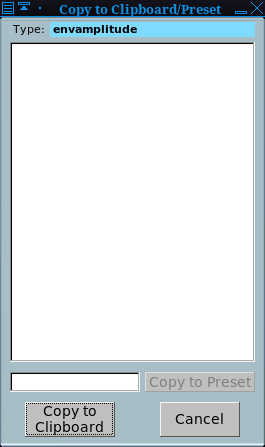
\includegraphics[scale=0.75]{bottom-panel/instrument-edit/ADD/copy-to-clipboard-preset.jpg}
   \caption[Copy to Clipboard]{Copy to Clipboard/Presets}
   \label{fig:copy_to_clipboard} 
\end{figure}

   \setcounter{ItemCounter}{0}      % Reset the ItemCounter for this list.

   \itempar{Type}{clipboard!copy type}
   Clipboard type for copying.
   This field indicates the context (e.g h. "envamplitude") or name of the
   clipboard to which the data will be copied.
   If the preset is saved/copied to a file, this
   field becomes the second part of the preset's file-name.

   \itempar{Clipboard list}{clipboard!list}
   Clipboard list.
   \index{preset!list}
   This itemm is actually a list of preset files available to be selected for
   this block of \textsl{Yoshimi} settings.

   \itempar{Copy to Preset}{preset!copy}
   Clipboard to preset.
   Provides a way to specify the preset (and, indirectly, the preset file)
   to which this data should be copied.

   To save to a preset, type the desired name of the setting.  This entry
   will enable this button.  When the button is pressed, the preset will
   be saved to the default preset directory.
   Be sure to set up a default present directory where ordinary users have write
   permissions!
   A good choice for a preset directory is
   \texttt{\textasciitilde/.config/yoshimi/presets}.
   \index{preset files!.ADnoteParameters.xpz}
   The file-name of the of the preset will be a non-hidden file such as

   \begin{verbatim}
      my_preset.ADnoteParameters.xpz
   \end{verbatim}

   The middle part of this name is shown near the top of the preset dialog, as
   a cue.
   There is no way in \textsl{Yoshimi} to change this part of the file-name.
   And don't do it using file system commands!  Modify the first part of the
   file-name to distinguish it from other versions of the preset.
   Only the type-name will ever be visible in the \textsl{Yoshimi}
   presets \textbf{Type} field.

   Note that \textsl{Yoshimi} ships with a number of non-hidden \texttt{.xpz}
   files.

   \itempar{Copy to Clipboard}{clipboard!copy}
   \index{preset!copy}
   Copies the preset to the clipboard.

\subsubsection{Clipboard/Preset Paste}
\label{subsubsec:clipboard_paste}

   \index{clipboard!paste}
   \index{preset!paste}
   Observe \figureref{fig:paste_to_clipboard}.
   It shows an example of the pasting dialog for the clipboard.

\begin{figure}[H]
   \centering 
   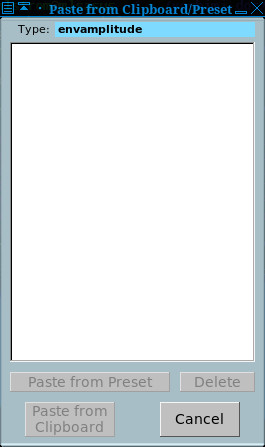
\includegraphics[scale=0.75]{bottom-panel/instrument-edit/ADD/paste-from-clipboard-preset.jpg}
   \caption[Paste from Clipboard]{Paste from Clipboard/Presets}
   \label{fig:paste_to_clipboard} 
\end{figure}

   \begin{enumber}
      \item \textbf{Add point}
      \item \textbf{Type}
      \item \textbf{Clipboard list}
      \item \textbf{Paste from Preset}
      \item \textbf{Paste from Clipboard}
   \end{enumber}

   \setcounter{ItemCounter}{0}      % Reset the ItemCounter for this list.

   \itempar{Type}{clipboard!paste type}
   Clipboard type for pasting.  
   This field indicates the context (e.g h. "envamplitude") or name of the
   clipboard to which the data will be copied.

   \itempar{Clipboard list}{clipboard!list}
   Clipboard list.

   \itempar{Paste from Preset}{preset!paste}
   Paste from preset.
   Provides a way to specify the preset to which this data should be
   copied.

   \itempar{Paste from Clipboard}{clipboard!paste}
   Clipboard to preset.

%-------------------------------------------------------------------------------
% vim: ts=3 sw=3 et ft=tex
%-------------------------------------------------------------------------------
